\documentclass{article}
\usepackage{geometry}
\usepackage{graphicx}
\usepackage{eso-pic}
\usepackage{tikz}
\usepackage{float}
\usepackage{background}
\usepackage[T1]{fontenc}
\usepackage[utf8]{inputenc} % Solo si usas LaTeX
\usepackage[spanish]{babel}
\usepackage[expansion=false]{microtype}
\usepackage{fancyhdr}
\usepackage{titlesec}
\usepackage{xcolor}
\usepackage{hyperref} %% hipervínculos
\usepackage{textcomp} %% para usar ' 
\usepackage{array}
%\usepackage{ragged2e} %justificación
\usepackage[dvipsnames]{xcolor} %color 
\usepackage{longtable} %% tablas largas
\setlength{\parindent}{0pt}
\setlength{\parskip}{0.8em}


%\pagestyle{empty}

%%-----------INICIO Enumeración de pagina--------%%
\pagestyle{fancy}
\fancyhf{} % Limpia encabezados y pies
\fancyfoot[R]{\thepage} % Número de página centrado en el pie
\renewcommand{\headrulewidth}{0pt} % Quita la línea del encabezado
\renewcommand{\footrulewidth}{0pt} % Sin línea en el pie
% Aplicar también a páginas con estilo plain
\fancypagestyle{plain}{
    \fancyhf{}
    \fancyfoot[R]{\thepage}
    \renewcommand{\headrulewidth}{0pt}
    \renewcommand{\footrulewidth}{0pt}
}
%%-----------FIN Enumeración de paginas--------%%

\backgroundsetup{
    scale=1,
    angle=0,
    opacity=0.15, % Transparencia
    contents={
        
\includegraphics[width=\paperwidth,height=\paperheight]{ImagenesFormato/fondo.jpg}
    }
}

%% --------- Color de secciones y niveles----

\definecolor{alldatum}{HTML}{000080} % Ejemplo de color

\newcommand{\centersection}[1]{%
  \begin{center}
    {\Large\bfseries\color{alldatum} #1}
  \end{center}
}


\begin{document}
%% --------- INICIO --- Redefinir color de secciones y niveles----%%
%Sección
\titleformat{\section}
{\normalfont\Large\bfseries\raggedright\color{alldatum}}
{\thesection}{2em}{}

% Subsección
\titleformat{\subsection}
{\normalfont\large\bfseries\raggedright\color{alldatum}}
{\thesubsection}{1em}{}

% Sub subsección
\titleformat{\subsubsection}
{\normalsize\bfseries\color{alldatum}}
{\thesubsubsection}{0.5em}{}

%% --------- FIN --- Redefinir color de secciones y niveles----%%


\pagestyle{empty}
%



% \begin{tikzpicture}[remember picture, overlay]
%   % 1. Coloca la imagen abarcando toda la hoja 
%   \node[inner sep=0pt, at=(current page.center)] {
%     
\includegraphics[width=\paperwidth, height=\paperheight]{ImagenesFormato/image1.jpg}
%   };

%   % 2. Coloca el texto en blanco exactamente en el centro de la página
%   \node[white, align=center] at (current page.center) {
%     {\Huge \textbf{Tu Texto Aquí}}
%   };
% \end{tikzpicture}


% \begin{tikzpicture}[remember picture,overlay]
% \AddToShipoutPictureBG*{%
%     \AtPageLowerLeft{%
%         
\includegraphics[width=\paperwidth,height=\paperheight]{ImagenesFormato/image1.jpg}
%     }%
% }

% \mbox{}
% % Texto sobre la imagen
% \node[
%     text=white,
%     font=\fontsize{18}{20}\selectfont\bfseries,
%     align=center,
%     text width=10cm
% ] at (current page.center)
% {
%     CuCo - Memoria Técnica
% };

% \end{tikzpicture}

\NoBgThispage
\thispagestyle{empty}
\mbox{}
\begin{tikzpicture}[remember picture,overlay]

% \node at (current page.center) {%
%     
\includegraphics[
%         width=\paperwidth,
%         height=\paperheight
%     ]{ImagenesFormato/image1.jpg}
% };

\node[inner sep=0pt] at (current page.center) {%
    
\includegraphics[
        width=\paperwidth,
        height=\paperheight
    ]{ImagenesFormato/image1.jpg}
};

\node[
    text=white,
    font=\fontsize{18}{20}\selectfont\bfseries,
    align=center,
    text width=10cm
] at (current page.center)
{
    CuCo - Manual Usabilidad
};

\end{tikzpicture}
\newpage

\pagestyle{fancy}
\setcounter{page}{1}
%%%----- avisos de confidencialidad -----
\section*{CONFIDENCIALIDAD}
%\justifying

Toda la información contenida en este documento es considerada confidencial y pertenece a \textbf{ALLDATUM BUSINESS S.A. de C.V.}

Su divulgación solamente deberá ser efectuada con la finalidad específica de evaluación de su contenido para la eventual aprobación y contratación de los servicios ofrecidos.

Asimismo, ninguna parte de este documento podrá ser reproducida, parcial o totalmente, por cualquier medio, sin la autorización expresa y por escrito de \textbf{ALLDATUM BUSINESS S.A. de C.V.}

Al recibir esta propuesta, usted está de acuerdo con este aviso de confidencialidad.

\newpage
\centersection{\centering Manual Usabilidad: Cuentas Contables}

 \vspace{4cm}
\begin{figure}[H]
    \centering
    
\includegraphics[width=0.8\textwidth]{CMI/CMILogo.png}
\end{figure}
 \vspace{4cm}
\begin{figure}[H]
    \centering
    
\includegraphics[width=0.8\textwidth]{CMI/CMILetras.png}
\end{figure}

%%-------- índice ------%%
\newpage
\renewcommand{\contentsname}{Tabla de Contenido}
\tableofcontents


%\pagestyle{plain}
%\setcounter{page}{1}

%% ############ Recorrido de Perspectiva
\section{Recorrido por Perspectiva de Cuentas Contables}

\begin{enumerate}

\item
    \begin{minipage}[t]{\linewidth}
        Ingresar a  \url{https://mdm.somoscmi.com:8443/ebx-authentication/login?resume=/ebx-iu/ui}
        \raggedright
        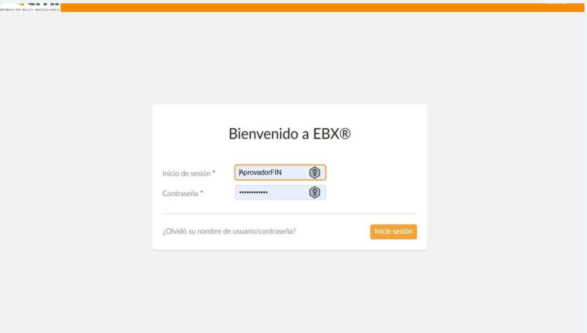
\includegraphics[width=0.8\textwidth]{RecorridoPerspectiva/ImgRecorridoPerspectiva/RP01.png}

    \end{minipage}

\item
    \begin{minipage}[t]{\linewidth}
        Click "Inicie sesión".
        \raggedright
        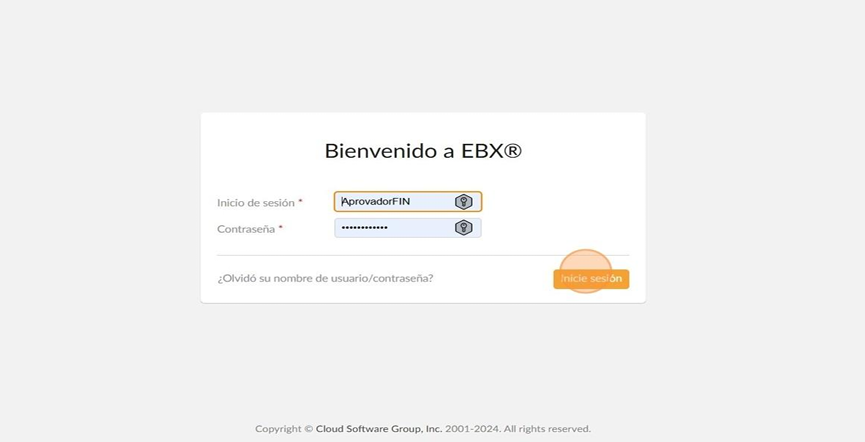
\includegraphics[width=0.8\textwidth]{RecorridoPerspectiva/ImgRecorridoPerspectiva/RP02.png}

    \end{minipage}    

\item
    \begin{minipage}[t]{\linewidth}
        Damos click "Bandeja de Entrada".
        \raggedright
        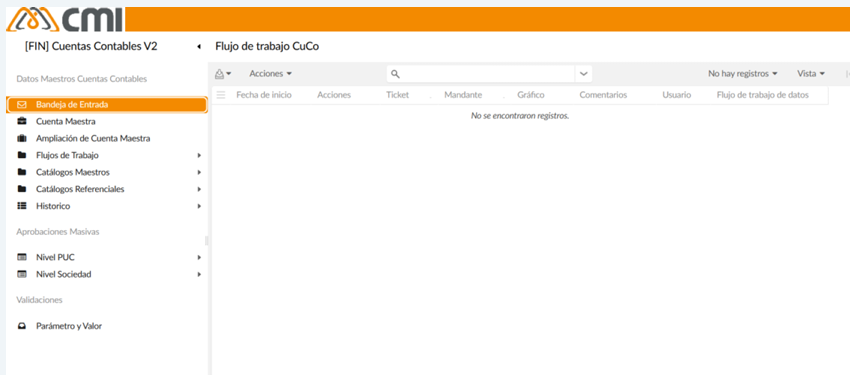
\includegraphics[width=0.8\textwidth]{RecorridoPerspectiva/ImgRecorridoPerspectiva/RP03.png}

    \end{minipage}  

\item
    \begin{minipage}[t]{\linewidth}
        Dentro de la Bandeja de Entrada están todos los flujos pendientes que tenga el usuario o el rol.

        \raggedright
        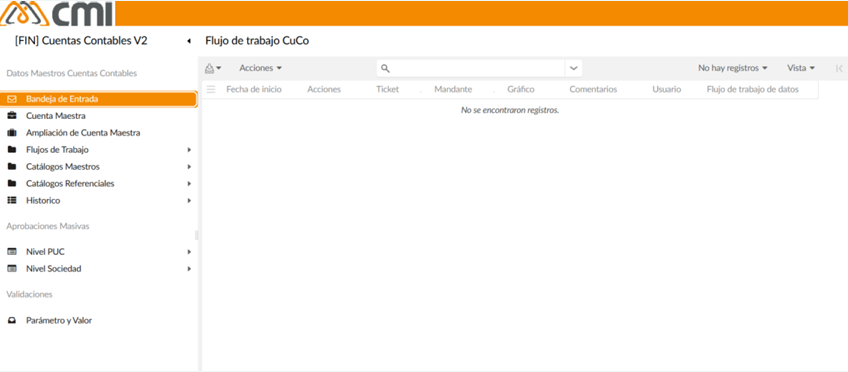
\includegraphics[width=0.8\textwidth]{RecorridoPerspectiva/ImgRecorridoPerspectiva/RP04.png}
    
    \end{minipage}  
 
\item
    \begin{minipage}[t]{\linewidth}
        Damos click "Cuenta Maestra”.
        \raggedright
        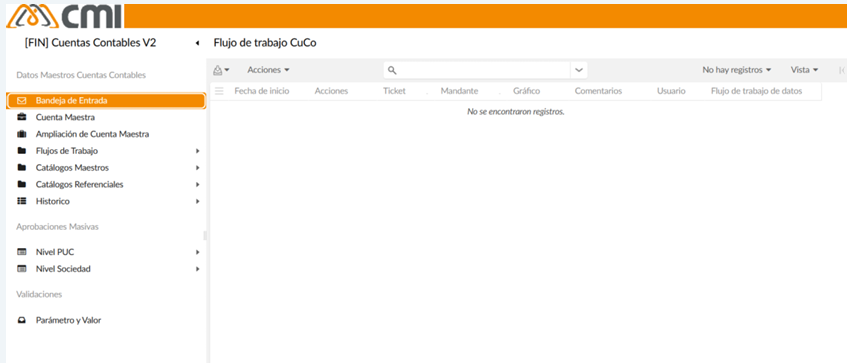
\includegraphics[width=0.8\textwidth]{RecorridoPerspectiva/ImgRecorridoPerspectiva/RP05.png}
    
    \end{minipage}

\item
    \begin{minipage}[t]{\linewidth}
        Dentro de Cuenta Maestra se encuentran las cuentas contables que se encuentran dentro SAP.
        
        Además de contar con botones que inicia el servicio creado para el dominio.
        \raggedright
        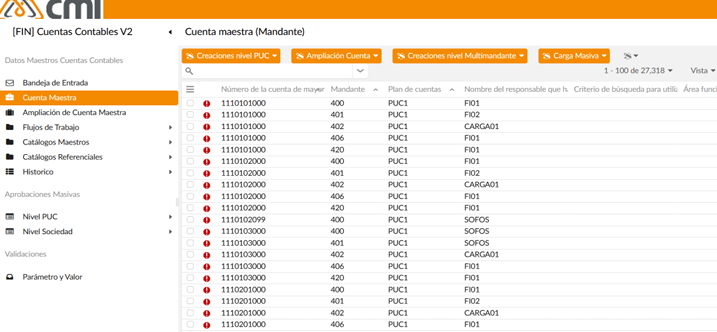
\includegraphics[width=0.8\textwidth]{RecorridoPerspectiva/ImgRecorridoPerspectiva/PR06.png}
    
    \end{minipage}      

    \item
    \begin{minipage}[t]{\linewidth}
        Damos click "Ampliación de Cuenta Maestra".
        \raggedright
        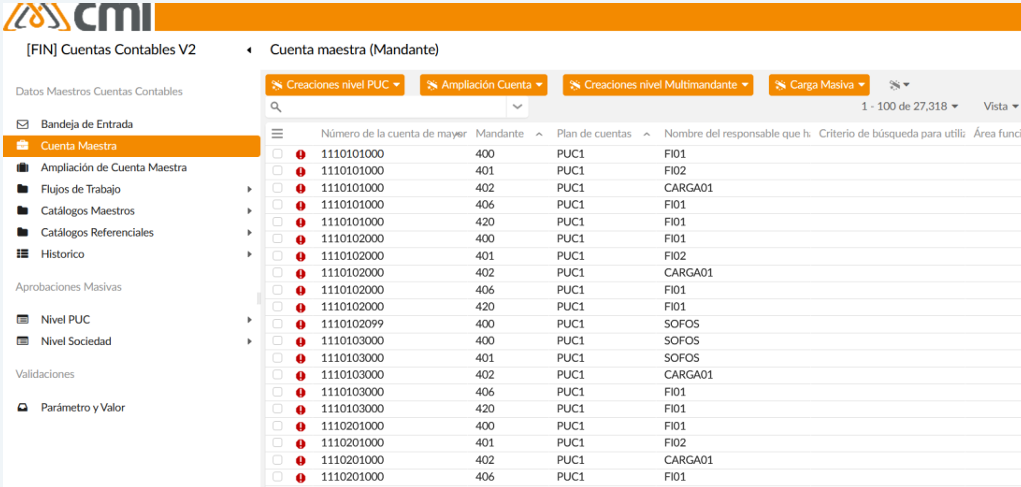
\includegraphics[width=0.8\textwidth]{RecorridoPerspectiva/ImgRecorridoPerspectiva/RP07.png}
   
    \end{minipage}   

    \item
    \begin{minipage}[t]{\linewidth}
        En Ampliación de cuenta Maestra, se encuentran las cuentas contables que están asociadas a una sociedad. 
        
        Adicional, se localizan los botones de acciones específicas para esta área.
        \raggedright
        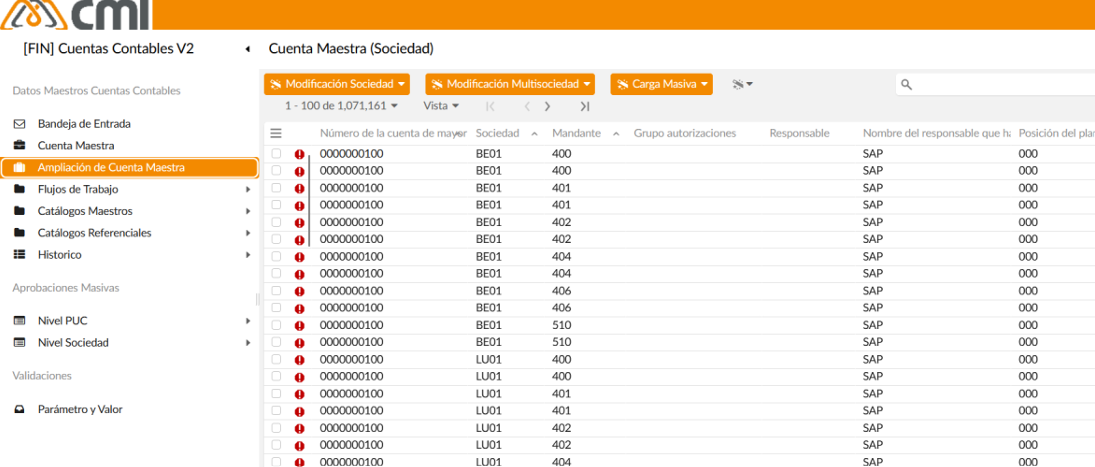
\includegraphics[width=0.8\textwidth]{RecorridoPerspectiva/ImgRecorridoPerspectiva/RP08.png}
     
    \end{minipage} 

     \item
    \begin{minipage}[t]{\linewidth}
        "Flujos de trabajo" es una lista desplegable que contiene apartados específicos para identificación de flujos de trabajo.
        
        \raggedright
        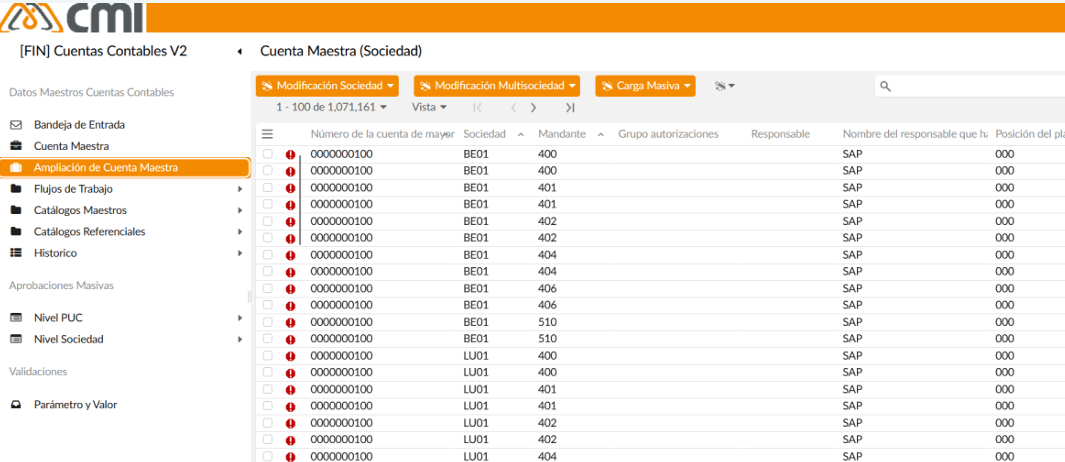
\includegraphics[width=0.8\textwidth]{RecorridoPerspectiva/ImgRecorridoPerspectiva/RP09.png}
     
    \end{minipage} 


    \item
    \begin{minipage}[t]{\linewidth}
        Dentro de "Flujos de Trabajo" se tienen 3 pestañas:
        \begin{itemize}
            \item Flujos de trabajo
            \item Flujos de trabajo activos
            \item Flujos de trabajo Completados
        \end{itemize}
        
        \raggedright
        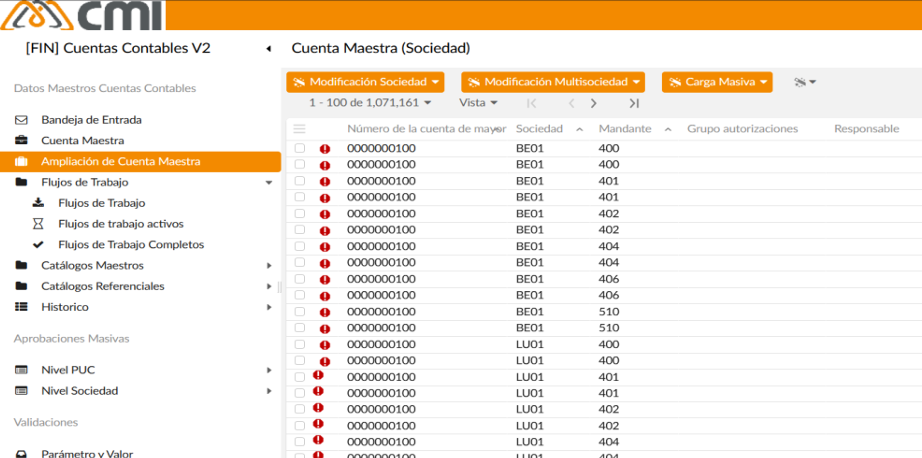
\includegraphics[width=0.8\textwidth]{RecorridoPerspectiva/ImgRecorridoPerspectiva/RP10.png}
     
    \end{minipage} 

    \item
    \begin{minipage}[t]{\linewidth}
        Dentro "Flujos de Trabajo" se tiene los flujos individuales del dominio por si es necesario una acción aislada.

        Cada flujo de trabajo tiene una etiqueta para su identificación.
        
        \raggedright
        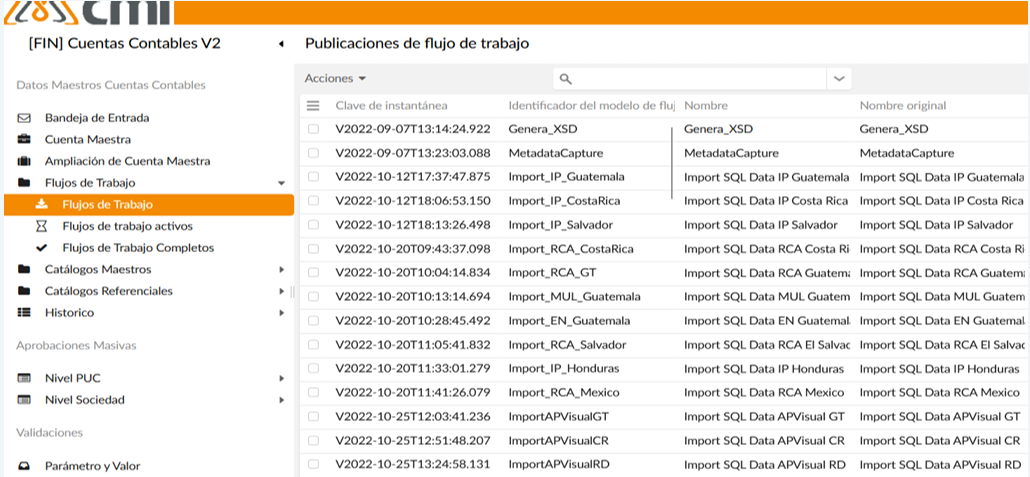
\includegraphics[width=0.8\textwidth]{RecorridoPerspectiva/ImgRecorridoPerspectiva/RP11.png}
     
    \end{minipage} 

    \item
    \begin{minipage}[t]{\linewidth}
        Si damos click en "Flujos de trabajo activos".
        
        \raggedright
        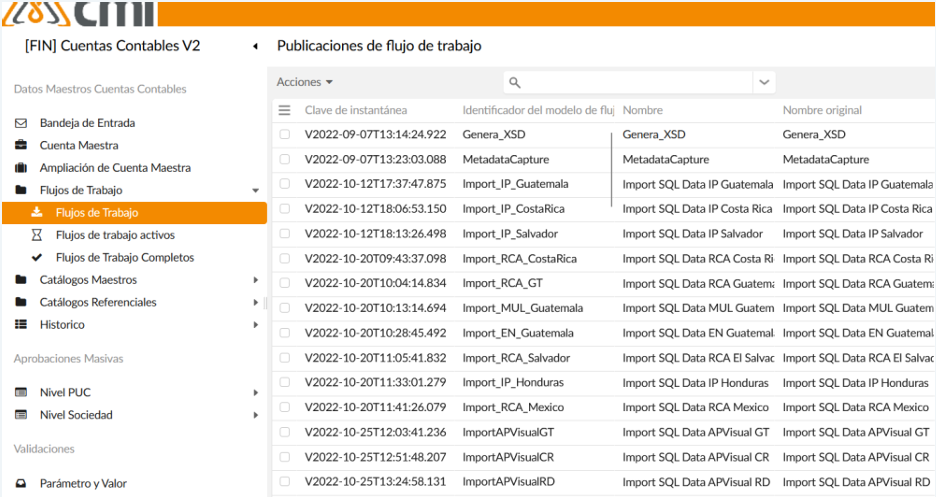
\includegraphics[width=0.8\textwidth]{RecorridoPerspectiva/ImgRecorridoPerspectiva/RP12.png}
     
    \end{minipage} 

    \item
    \begin{minipage}[t]{\linewidth}
        Dentro "Flujos de trabajo Activos" se muestra todos los flujos activos ya sea Creación / Modificación / Bloqueo / Ampliación, con su respectivo ticket y etiqueta del flujo en cuestión.
        
        \raggedright
        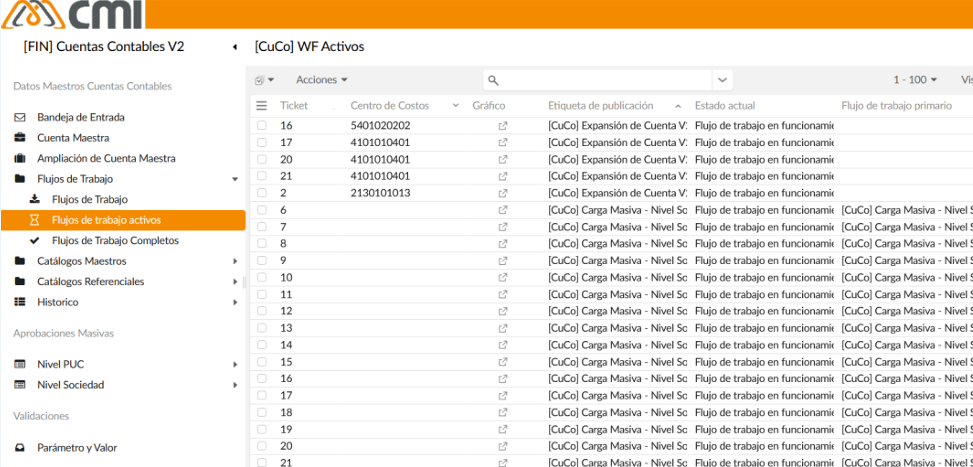
\includegraphics[width=0.8\textwidth]{RecorridoPerspectiva/ImgRecorridoPerspectiva/RP13.png}
     
    \end{minipage} 

    \item
    \begin{minipage}[t]{\linewidth}
        Si damos click en "Flujos de Trabajo Completos".
        
        \raggedright
        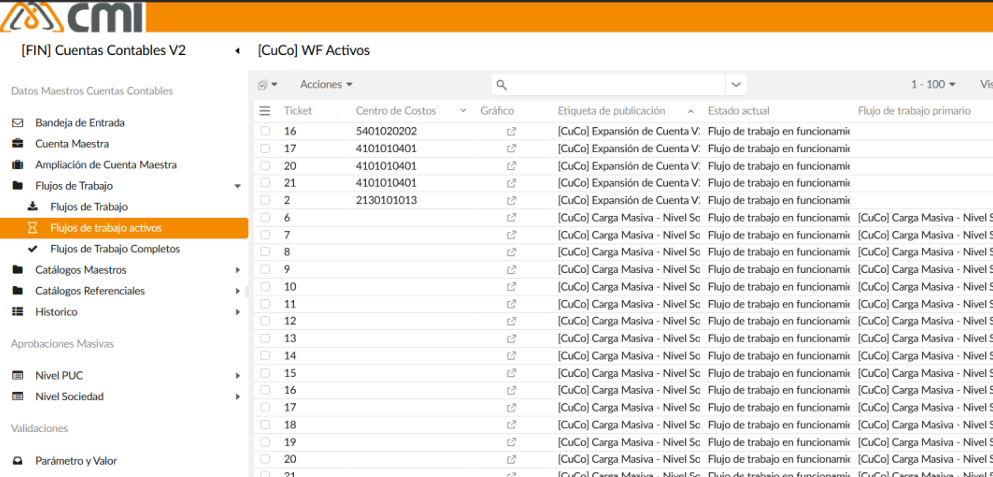
\includegraphics[width=0.8\textwidth]{RecorridoPerspectiva/ImgRecorridoPerspectiva/RP14.png}
     
    \end{minipage} 

    \item
    \begin{minipage}[t]{\linewidth}
        En "Flujos de Trabajo Completos" se encuentran todos los flujos que concluyeron para un análisis de cuales personas participaron en el flujo si es necesario.
        
        \raggedright
        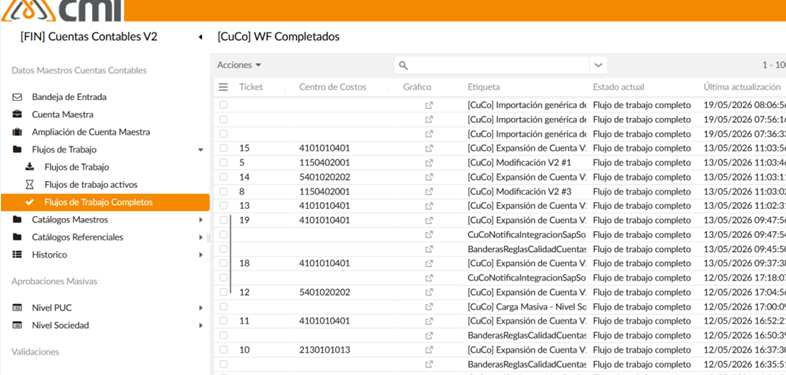
\includegraphics[width=0.8\textwidth]{RecorridoPerspectiva/ImgRecorridoPerspectiva/RP15.png}
     
    \end{minipage}
    
    \item
    \begin{minipage}[t]{\linewidth}
        "Catálogos Maestros" es otra lista que contiene todos los catálogos utilizados dentro el dominio.
        
        \raggedright
        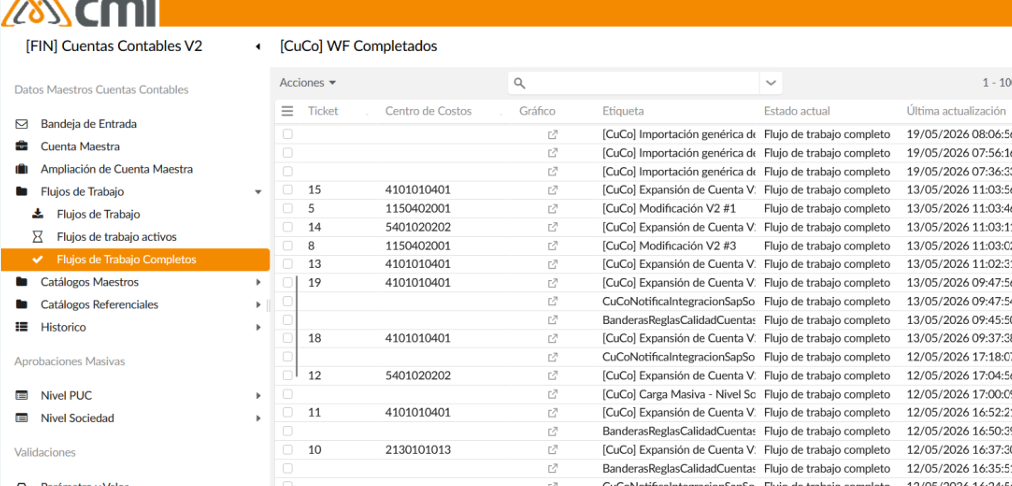
\includegraphics[width=0.8\textwidth]{RecorridoPerspectiva/ImgRecorridoPerspectiva/RP16.png}
     
    \end{minipage} 

    \item
    \begin{minipage}[t]{\linewidth}
        Damos click en "Mandante".
        
        \raggedright
        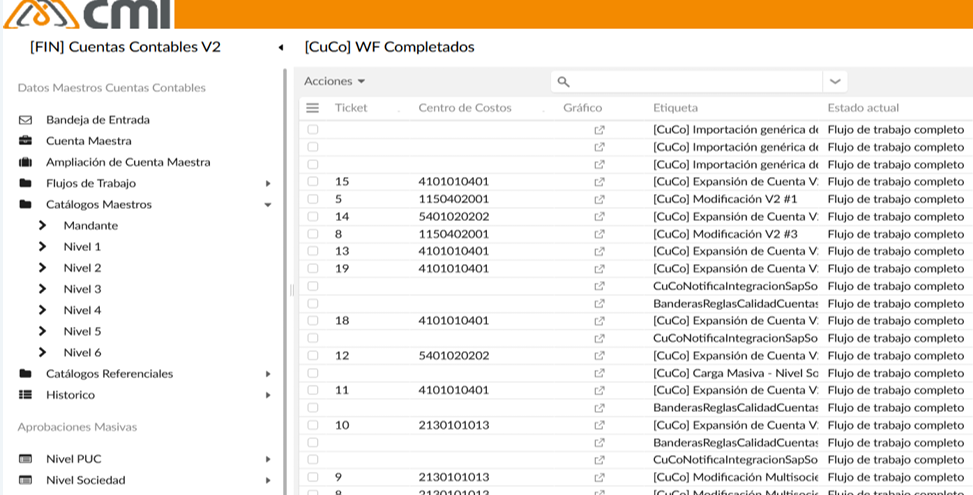
\includegraphics[width=0.8\textwidth]{RecorridoPerspectiva/ImgRecorridoPerspectiva/RP17.png}
     
    \end{minipage} 

    \item
    \begin{minipage}[t]{\linewidth}
        Se encuentran todos los mandantes asociados a los servicios desarrollados.
        
        \raggedright
        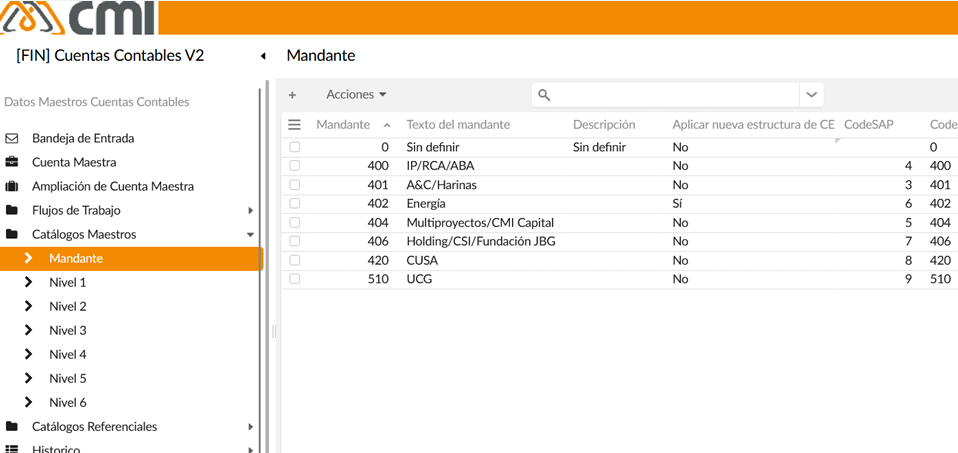
\includegraphics[width=0.8\textwidth]{RecorridoPerspectiva/ImgRecorridoPerspectiva/RP18.png}
     
    \end{minipage} 

    \item
    \begin{minipage}[t]{\linewidth}
        Si damos click en "Nivel 1".
        
        \raggedright
        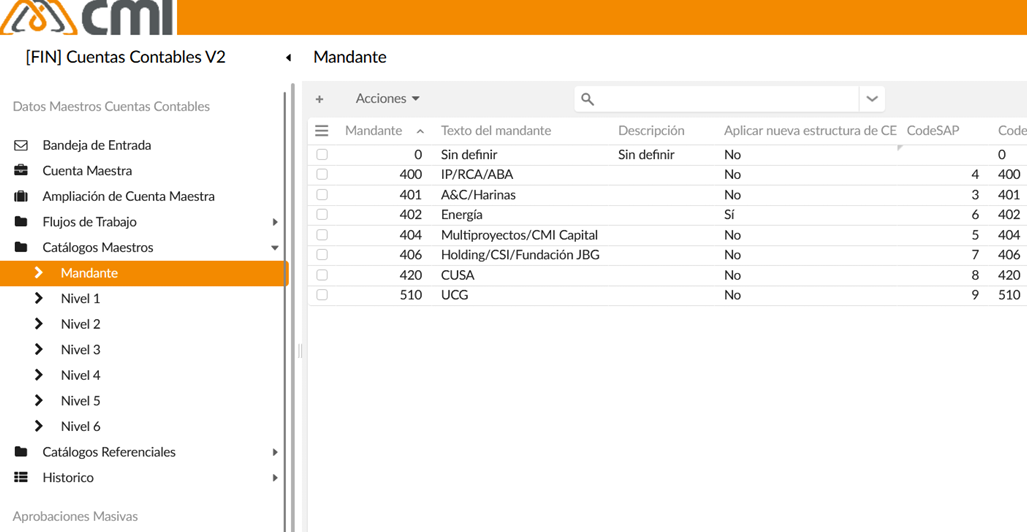
\includegraphics[width=0.8\textwidth]{RecorridoPerspectiva/ImgRecorridoPerspectiva/RP19.png}
     
    \end{minipage} 

    \item
    \begin{minipage}[t]{\linewidth}
        Dentro de "Nivel 1" se encuentra el catálogo al primer nivel de una cuenta contable.
        
        \raggedright
        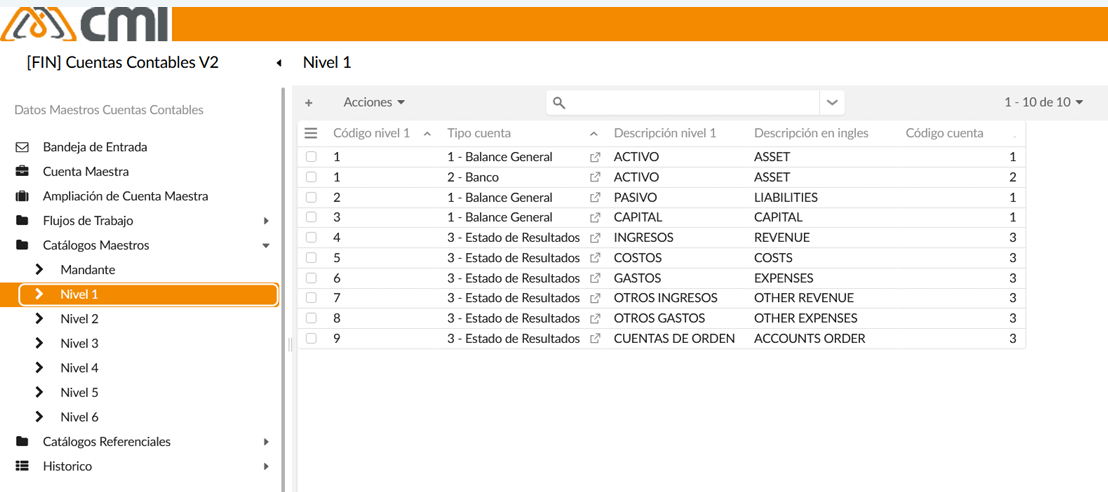
\includegraphics[width=0.8\textwidth]{RecorridoPerspectiva/ImgRecorridoPerspectiva/RP20.png}
     
    \end{minipage} 


    \item
    \begin{minipage}[t]{\linewidth}
        Dentro de "Nivel 2" se encuentra el catálogo al primer nivel de una cuenta contable.
        
        \raggedright
        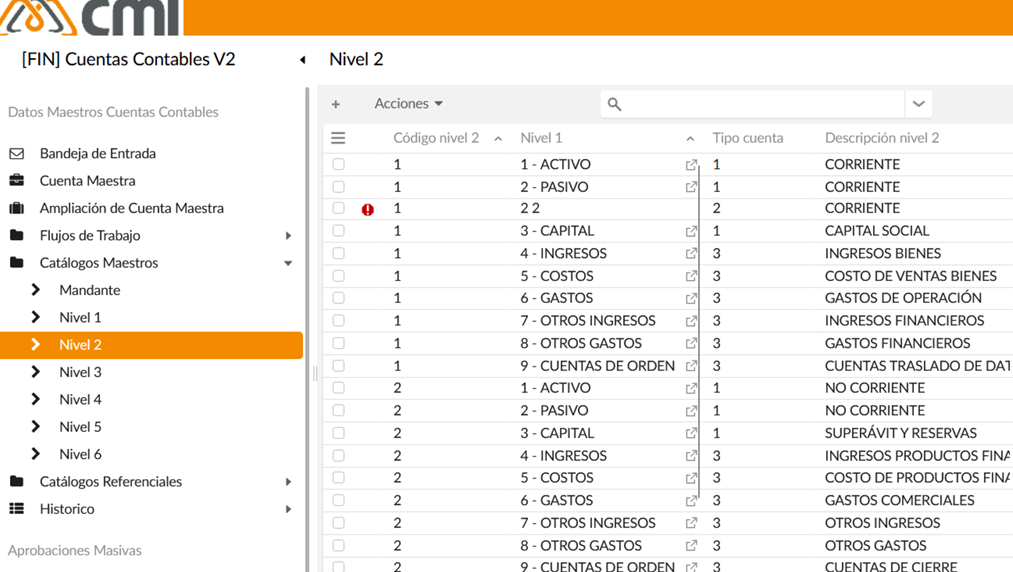
\includegraphics[width=0.8\textwidth]{RecorridoPerspectiva/ImgRecorridoPerspectiva/RP21.png}
     
    \end{minipage} 

    \item
    \begin{minipage}[t]{\linewidth}
        Dentro de "Nivel 3" se encuentra el catálogo al tercer nivel de una cuenta contable.
        
        \raggedright
        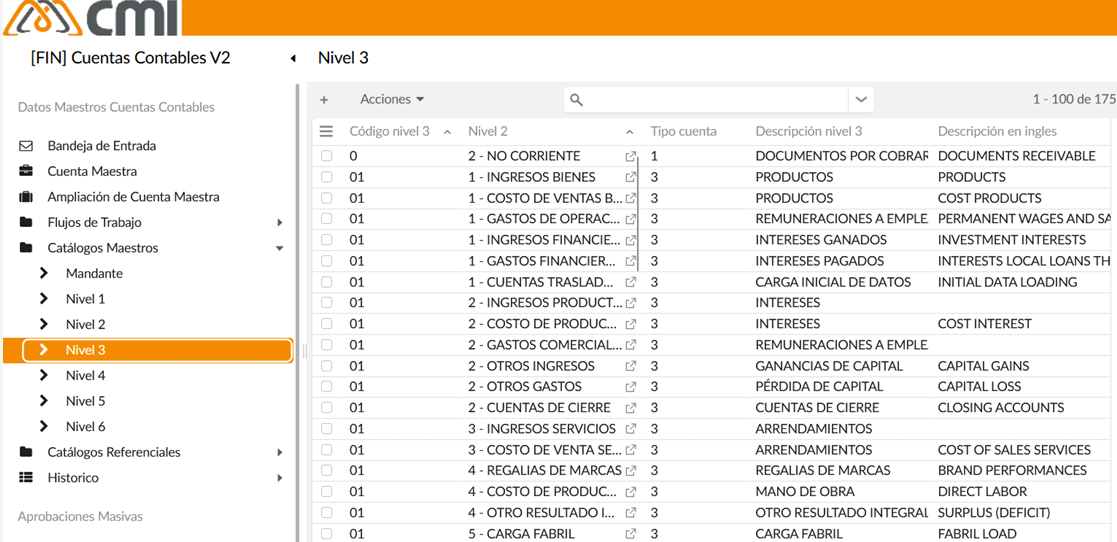
\includegraphics[width=0.8\textwidth]{RecorridoPerspectiva/ImgRecorridoPerspectiva/RP22.png}
     
    \end{minipage}

    \item
    \begin{minipage}[t]{\linewidth}
        Dentro de "Nivel 4" se encuentra el catálogo al cuarto nivel de una cuenta contable.
        
        \raggedright
        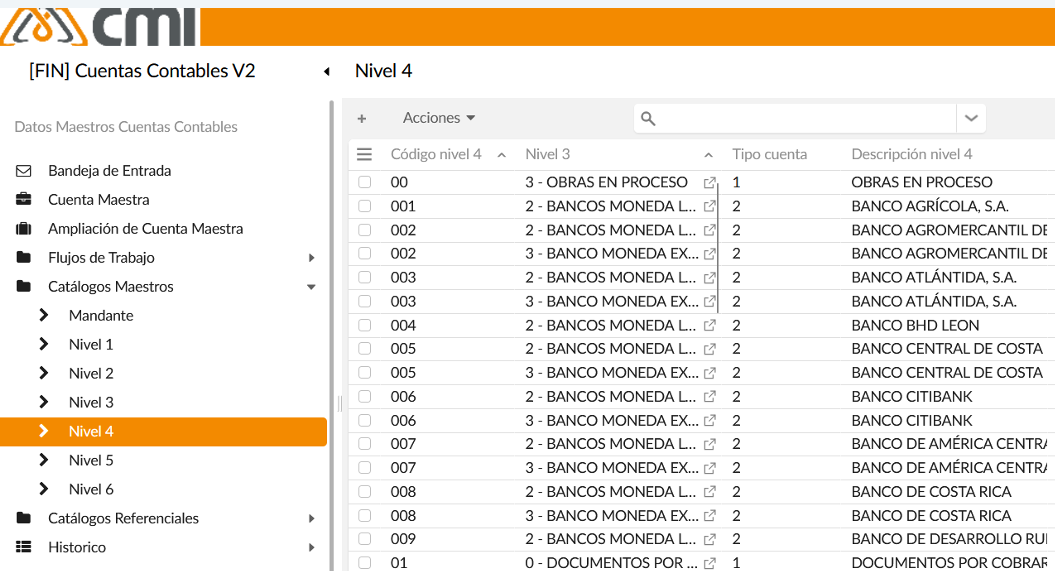
\includegraphics[width=0.8\textwidth]{RecorridoPerspectiva/ImgRecorridoPerspectiva/RP23.png}
     
    \end{minipage}

    \item
    \begin{minipage}[t]{\linewidth}
        Dentro de "Nivel 5" se encuentra el catálogo al quinto nivel de una cuenta contable.
        
        \raggedright
        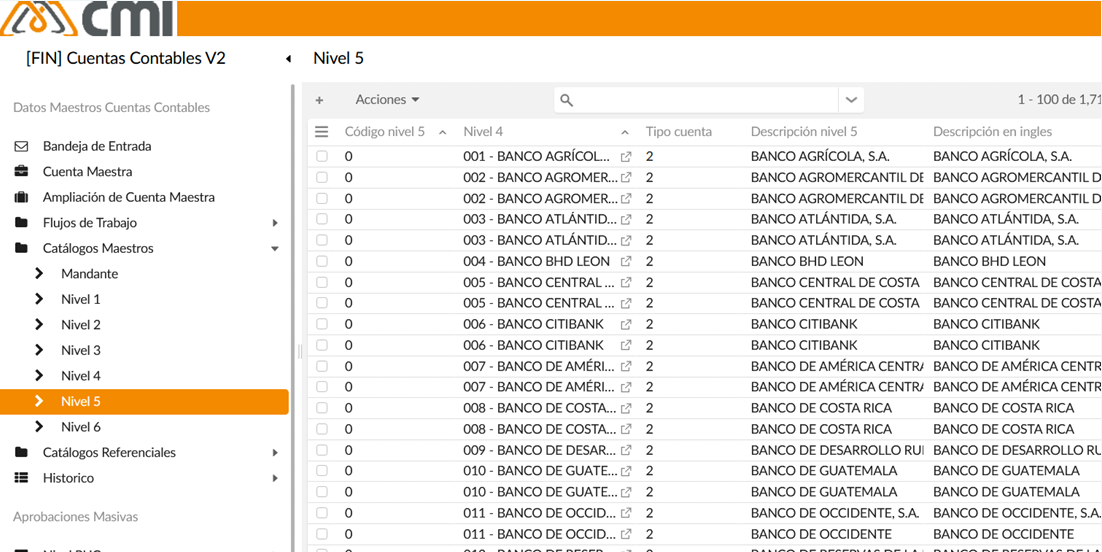
\includegraphics[width=0.8\textwidth]{RecorridoPerspectiva/ImgRecorridoPerspectiva/RP24.png}
     
    \end{minipage}

    \item
    \begin{minipage}[t]{\linewidth}
        Dentro de "Nivel 6" se encuentra el catálogo al sexto nivel de una cuenta contable.
        
        \raggedright
        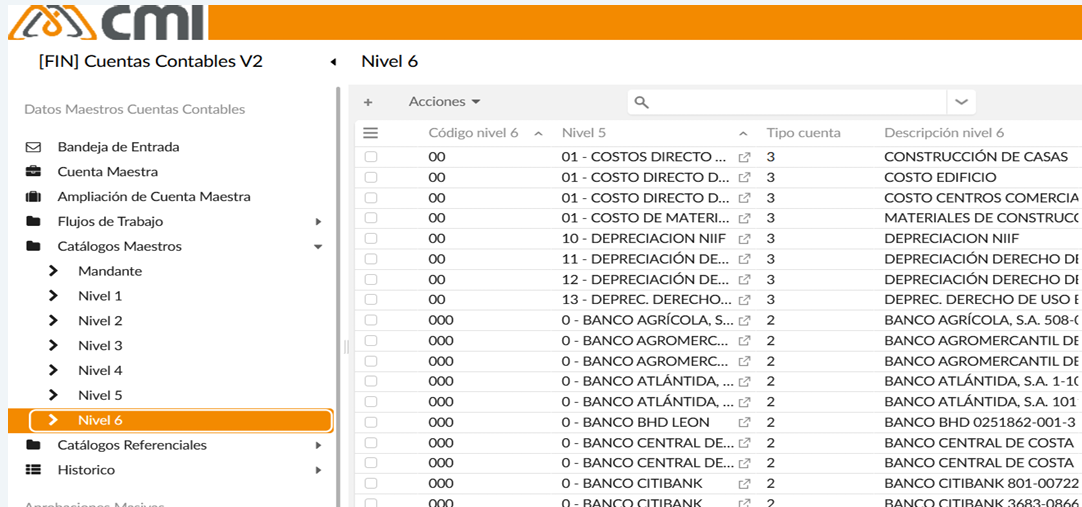
\includegraphics[width=0.8\textwidth]{RecorridoPerspectiva/ImgRecorridoPerspectiva/RP25.png}
     
    \end{minipage}


    \item
    \begin{minipage}[t]{\linewidth}
        Si damos click en "Parámetro y Valor".

        \raggedright
        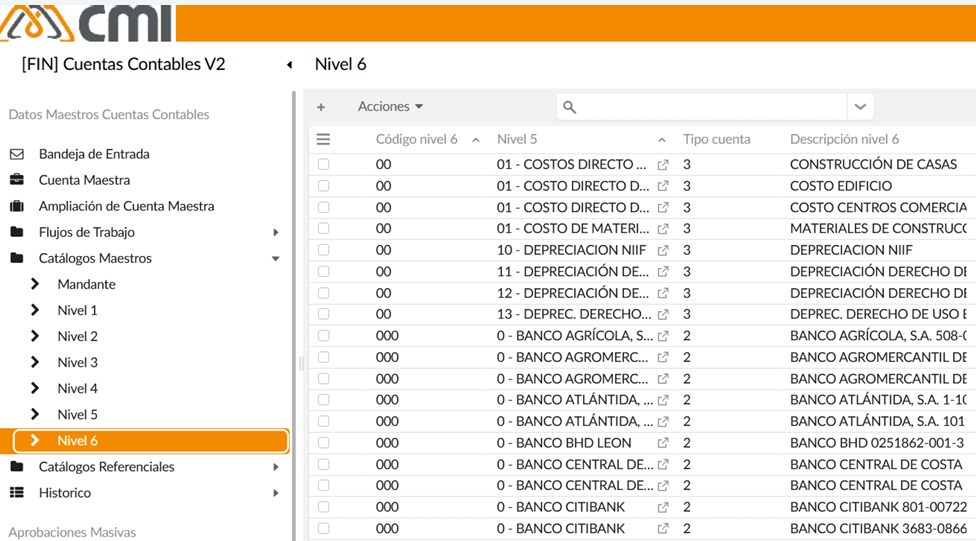
\includegraphics[width=0.8\textwidth]{RecorridoPerspectiva/ImgRecorridoPerspectiva/RP26.png}
     
    \end{minipage}
%%-----
    \item
    \begin{minipage}[t]{\linewidth}
        Si damos click en "Parámetro y Valor".

        \raggedright
        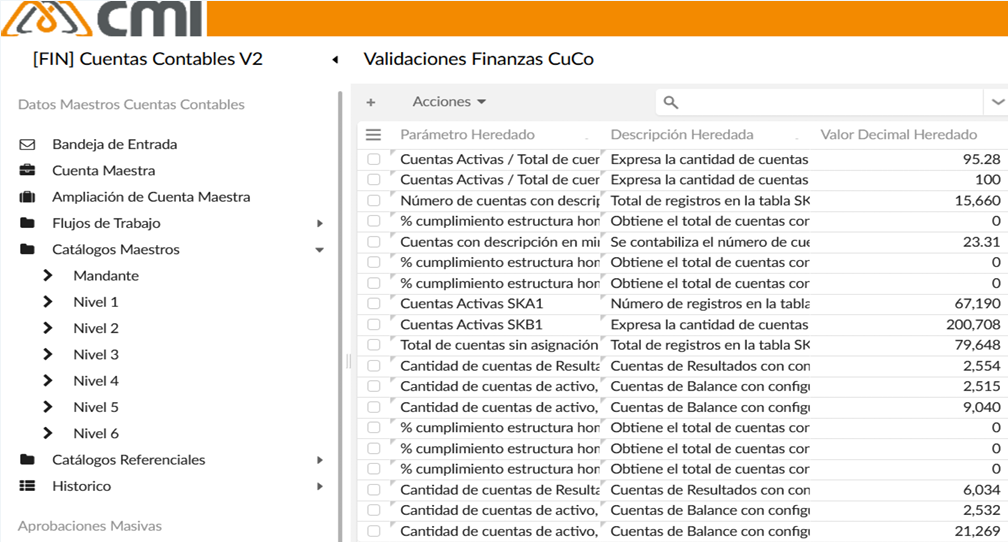
\includegraphics[width=0.8\textwidth]{RecorridoPerspectiva/ImgRecorridoPerspectiva/RP27.png}
     
    \end{minipage}

    \item
    \begin{minipage}[t]{\linewidth}
        Click "Parámetro y Valor".

        \raggedright
        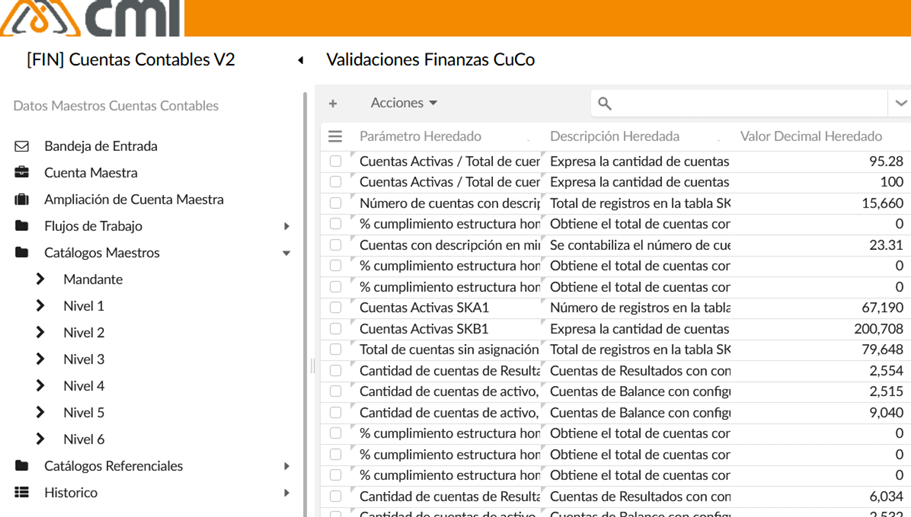
\includegraphics[width=0.8\textwidth]{RecorridoPerspectiva/ImgRecorridoPerspectiva/RP28.png}
     
    \end{minipage}

    \item
    \begin{minipage}[t]{\linewidth}
        Se muestra una tabla que contiene los resultados generales de las reglas de calidad.

        \raggedright
        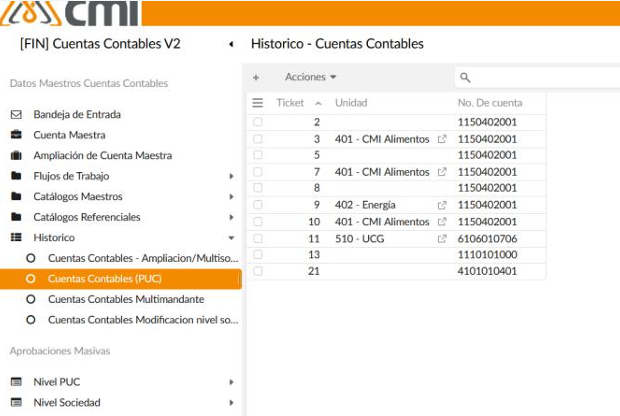
\includegraphics[width=0.8\textwidth]{RecorridoPerspectiva/ImgRecorridoPerspectiva/RP29.png}
     
    \end{minipage}

    \item
    \begin{minipage}[t]{\linewidth}
        En el apartado de Histórico se puede ver un espacio de registros y cambios realizados a una cuenta finalizada o en proceso. El área se divide en:

        \begin{itemize}
            \item Ampliación/Multi sociedad
            \item Nivel PUC
            \item Multi mandante
            \item Modificación a nivel sociedad
        \end{itemize}

        \raggedright
        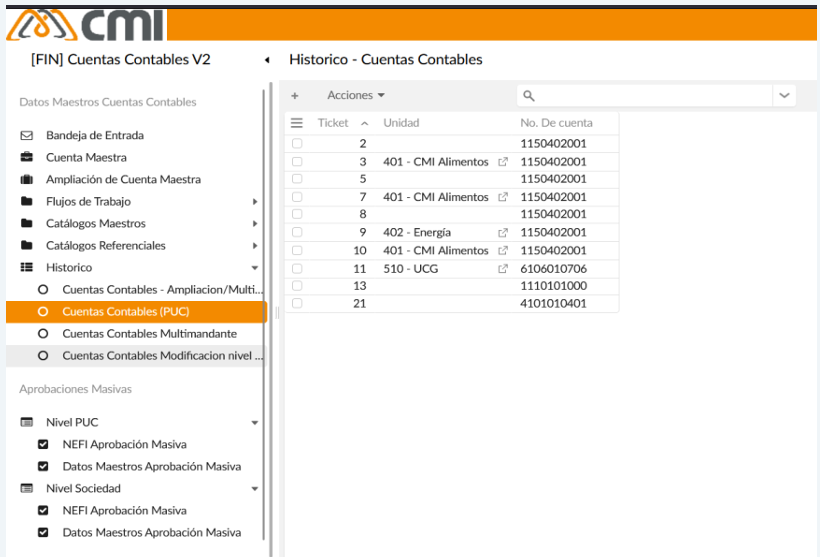
\includegraphics[width=0.6\textwidth]{RecorridoPerspectiva/ImgRecorridoPerspectiva/RP30.png}
     
    \end{minipage}

    \item
    \begin{minipage}[t]{\linewidth}
        En el área de Aprobaciones masivas se encuentran las tablas para procesos de funcionalidad Masiva, en su respectivo apartado se mostrará mejor su funcionamiento.

        \raggedright
        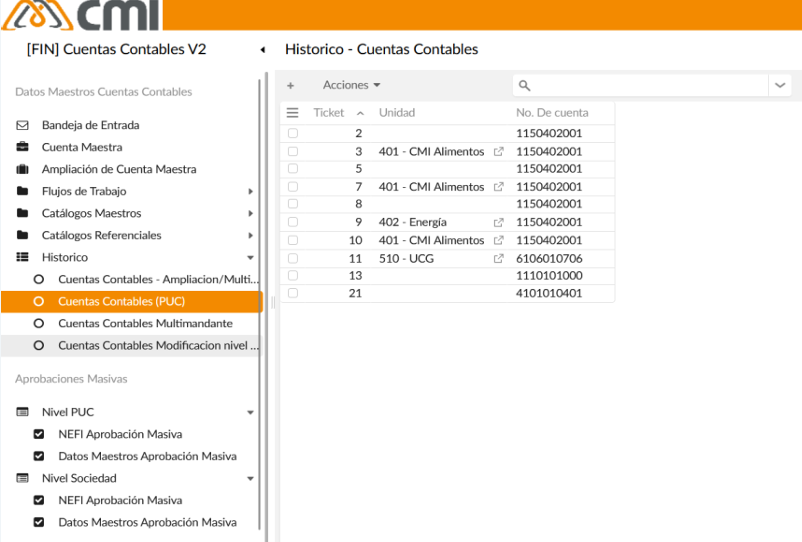
\includegraphics[width=0.8\textwidth]{RecorridoPerspectiva/ImgRecorridoPerspectiva/RP31.png}
     
    \end{minipage}





\end{enumerate}

%% Nivel PUC
\section{Cuentas Contables - Nivel PUC}

%% ######## Creacion simple

\subsection{Creación de Cuenta Contable}

\begin{enumerate}

\item
    \begin{minipage}[t]{\linewidth}
        Ingresar a  \url{https://mdm.somoscmi.com:8443/ebx-ui/ui/custom/Cuentas/action/305}
        \raggedright
        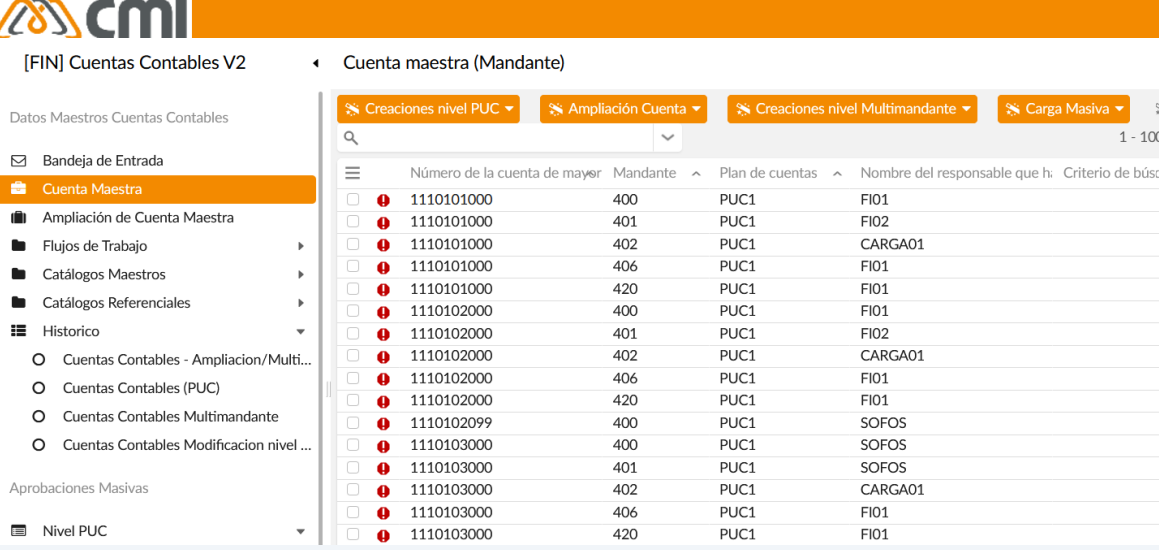
\includegraphics[width=0.8\textwidth]{NivelPUC/Creacion/ImgCreacion/CS01.png}

    \end{minipage}

\item
    \begin{minipage}[t]{\linewidth}
       Dentro de "Cuenta maestra" se ubica el servicio de creación de cuenta a nivel PUC. \raggedright
        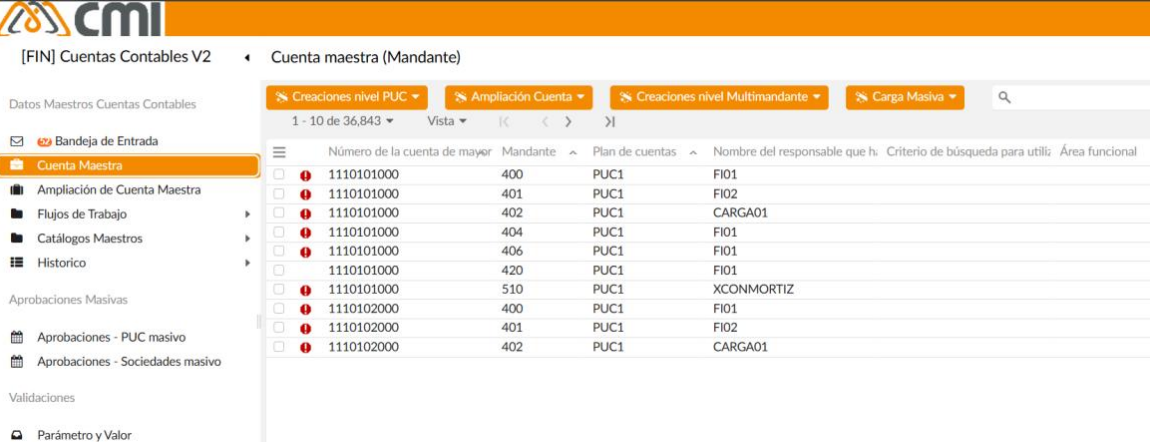
\includegraphics[width=0.8\textwidth]{NivelPUC/Creacion/ImgCreacion/CS02.png}

    \end{minipage}

\item
    \begin{minipage}[t]{\linewidth}
        Para iniciar una creación a nivel PUC se da click en "Creación Cuenta"

        \raggedright
        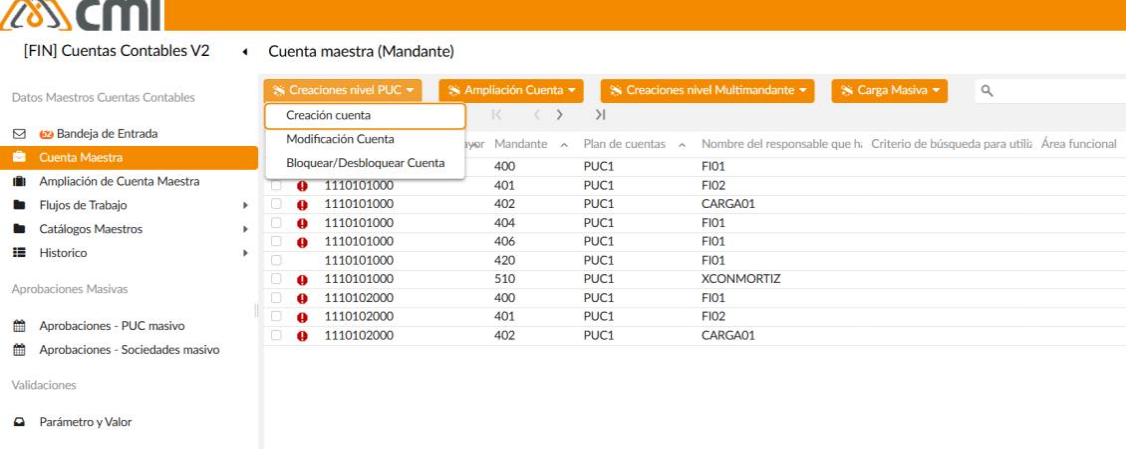
\includegraphics[width=0.8\textwidth]{NivelPUC/Creacion/ImgCreacion/CS03.png}

    \end{minipage}

\item
    \begin{minipage}[t]{\linewidth}
        Lo cual despliega un mensaje de confirmación para iniciar la creación de una cuenta.
        \raggedright
        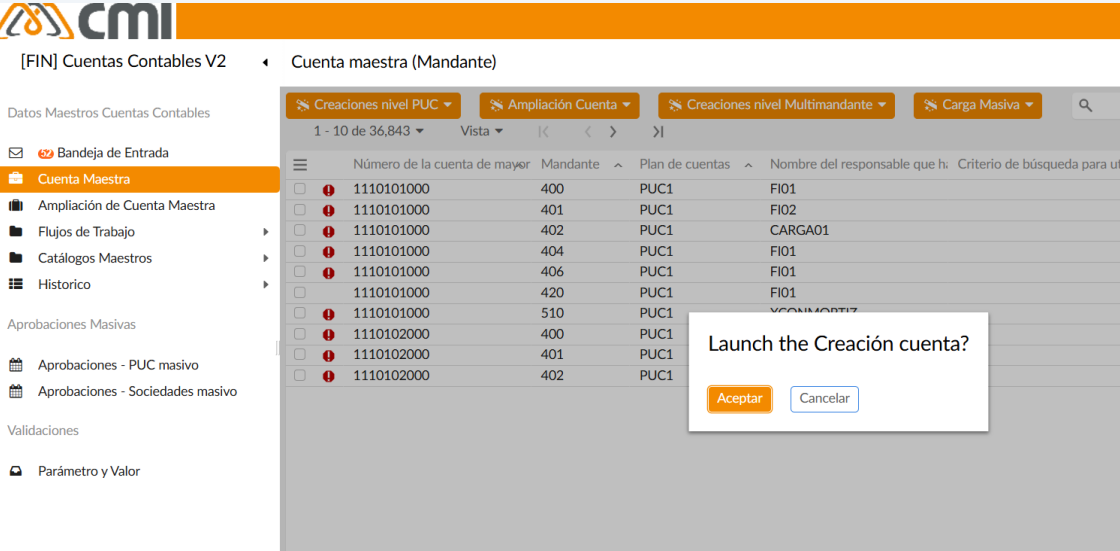
\includegraphics[width=0.8\textwidth]{NivelPUC/Creacion/ImgCreacion/CS04.png}

    \end{minipage}

\item
    \begin{minipage}[t]{\linewidth}
        Se despliega una pantalla donde se llevará a cabo el proceso de creación.

        \raggedright
        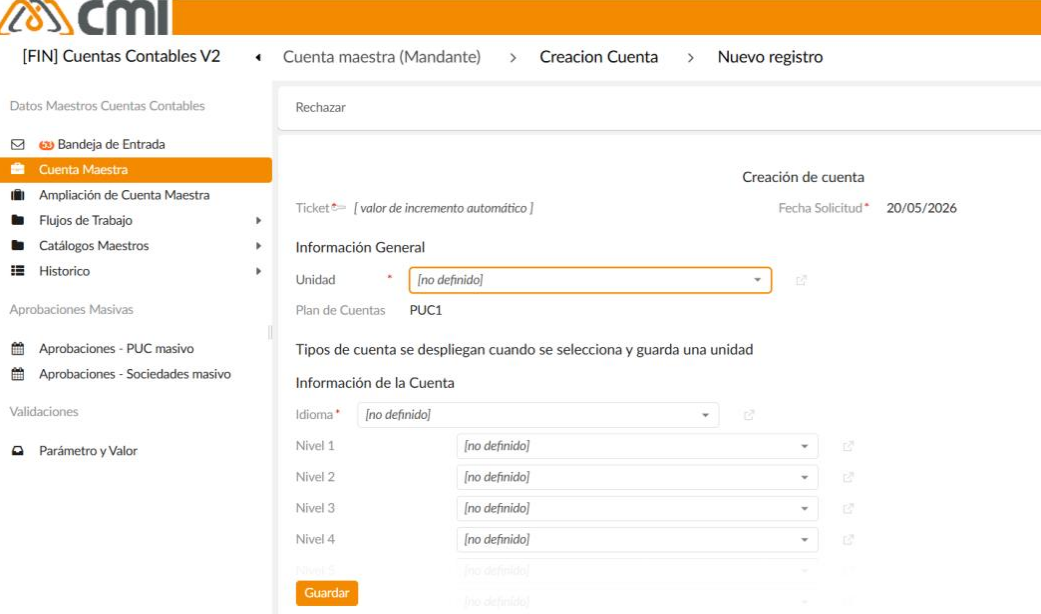
\includegraphics[width=0.8\textwidth]{NivelPUC/Creacion/ImgCreacion/CS05.png}

    \end{minipage}

\item
    \begin{minipage}[t]{\linewidth}
        001 - Vista del formulario de creación.

        \raggedright
        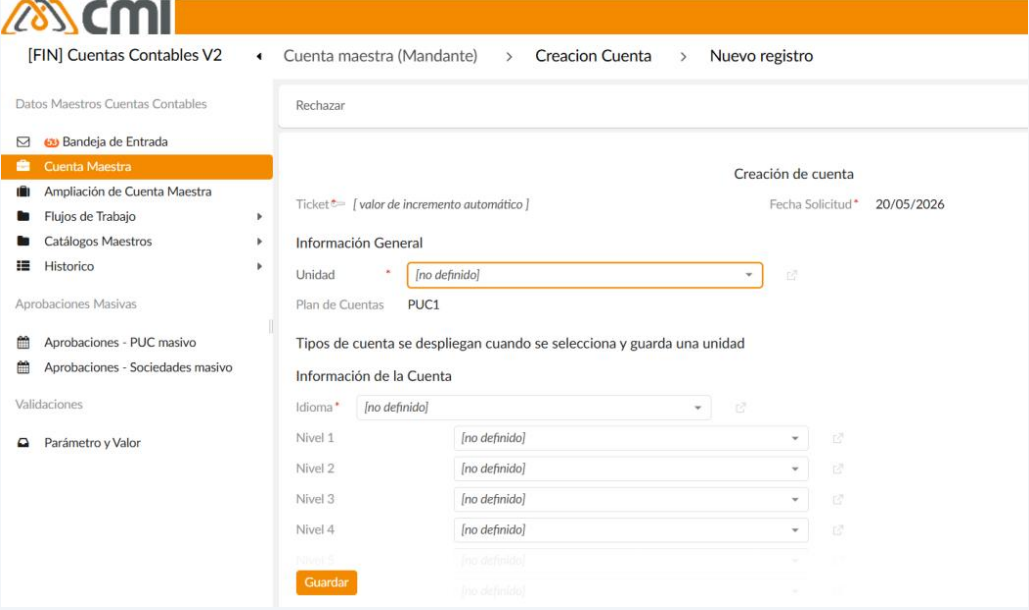
\includegraphics[width=0.8\textwidth]{NivelPUC/Creacion/ImgCreacion/CS06.png}

    \end{minipage}

\item
    \begin{minipage}[t]{\linewidth}
        Dentro el formulario se selecciona una unidad y al guardar aparece el tipo de cuenta a crear:

        \raggedright
        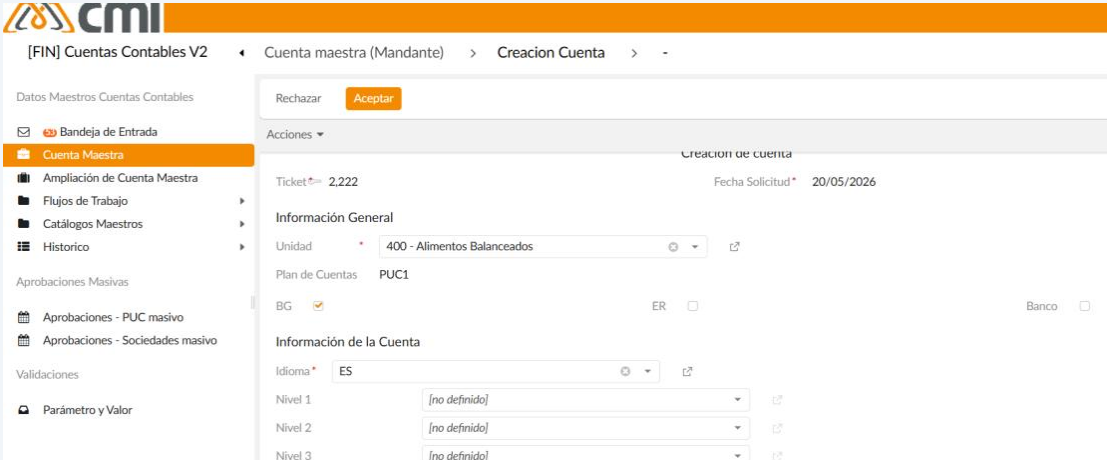
\includegraphics[width=0.8\textwidth]{NivelPUC/Creacion/ImgCreacion/CS07.png}

    \end{minipage}

\item
    \begin{minipage}[t]{\linewidth}
        \begin{itemize}
            \item BG: Balance General 
            \item ER: Estado de Resultados 
            \item Banco
        \end{itemize}
        
        \raggedright
        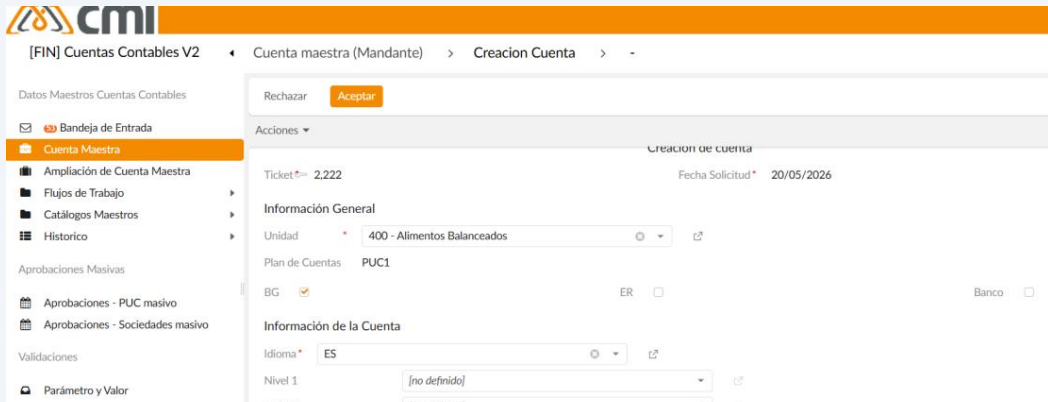
\includegraphics[width=0.8\textwidth]{NivelPUC/Creacion/ImgCreacion/CS08.png}

    \end{minipage}

\item
    \begin{minipage}[t]{\linewidth}
        Dentro el campo de unidad esta la lista de los mandantes y unidades disponibles.

        \raggedright
        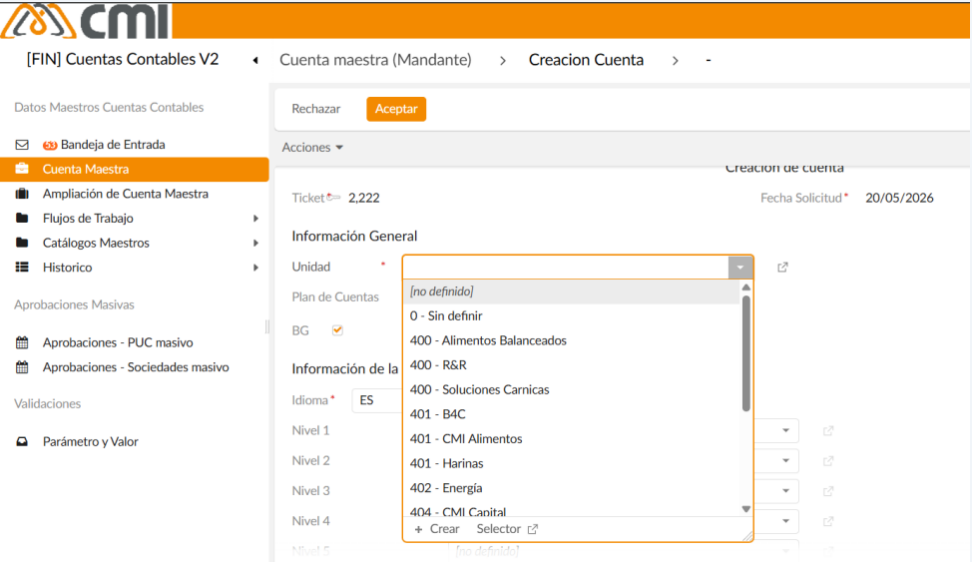
\includegraphics[width=0.8\textwidth]{NivelPUC/Creacion/ImgCreacion/CS09.png}

    \end{minipage}

\item
    \begin{minipage}[t]{\linewidth}
        Como siguiente paso se elige el tipo de idioma de la cuenta contable.

        \raggedright
        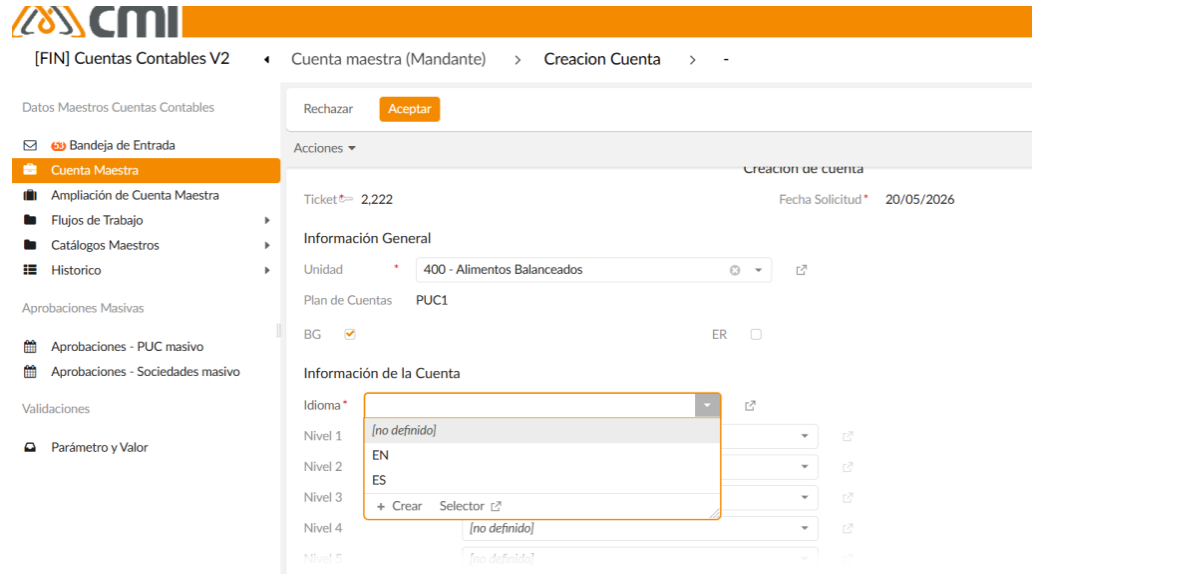
\includegraphics[width=0.8\textwidth]{NivelPUC/Creacion/ImgCreacion/CS10.png}

    \end{minipage}

\item
    \begin{minipage}[t]{\linewidth}
        En consiguiente se seleccionarán los niveles correctos para crear la cuenta contable.

        \raggedright
        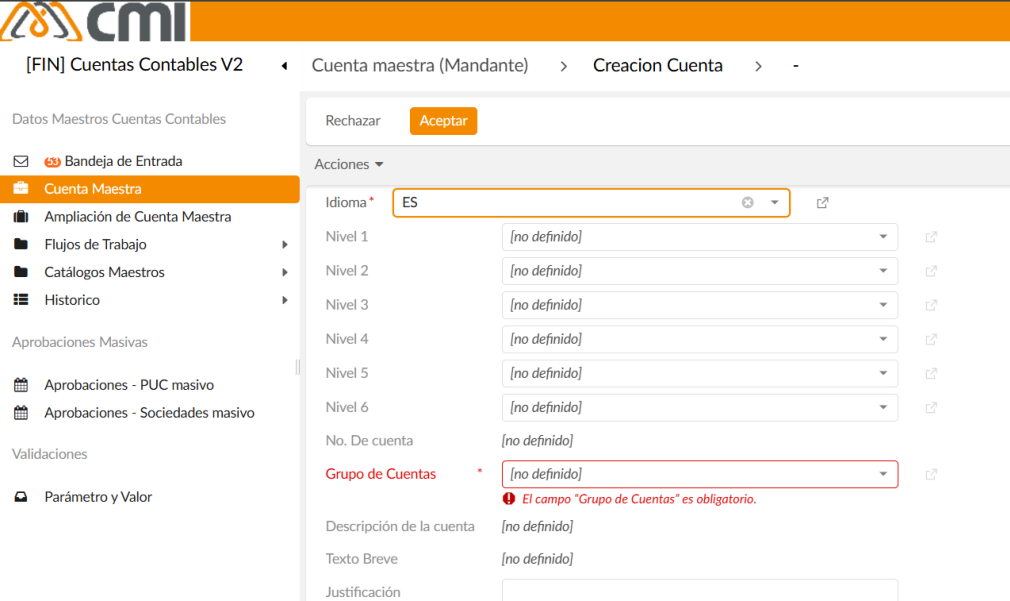
\includegraphics[width=0.8\textwidth]{NivelPUC/Creacion/ImgCreacion/CS11.png}

    \end{minipage}

\item
    \begin{minipage}[t]{\linewidth}
       Dentro el catálogo de "Nivel 1" se elige la opción correspondiente.

        \raggedright
        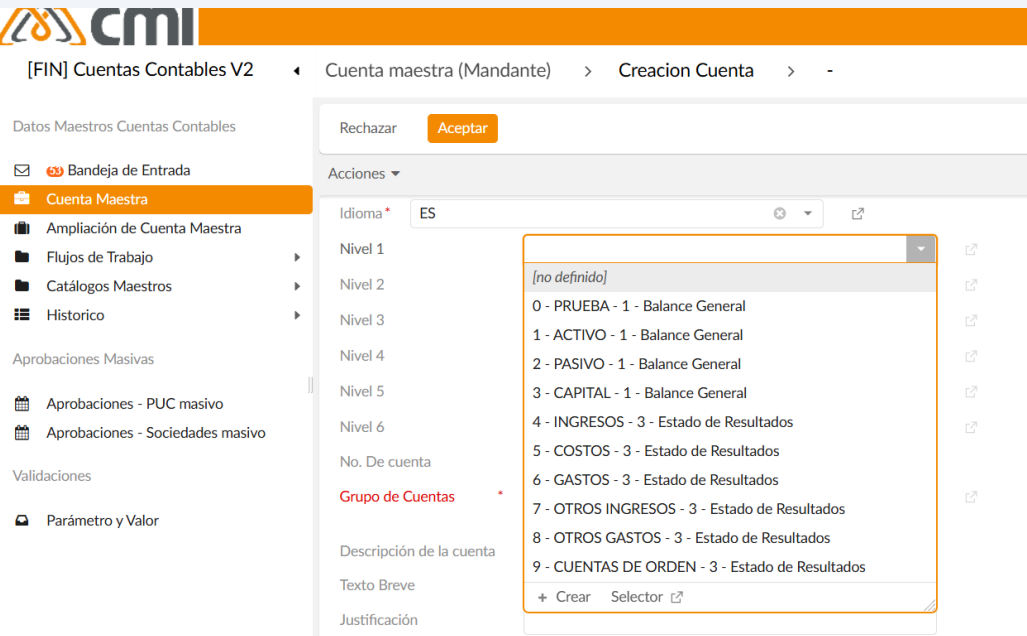
\includegraphics[width=0.8\textwidth]{NivelPUC/Creacion/ImgCreacion/CS12.png}

    \end{minipage}

\item
    \begin{minipage}[t]{\linewidth}
        Dentro el catálogo de "Nivel 2" se elige la opción correspondiente.

        \raggedright
        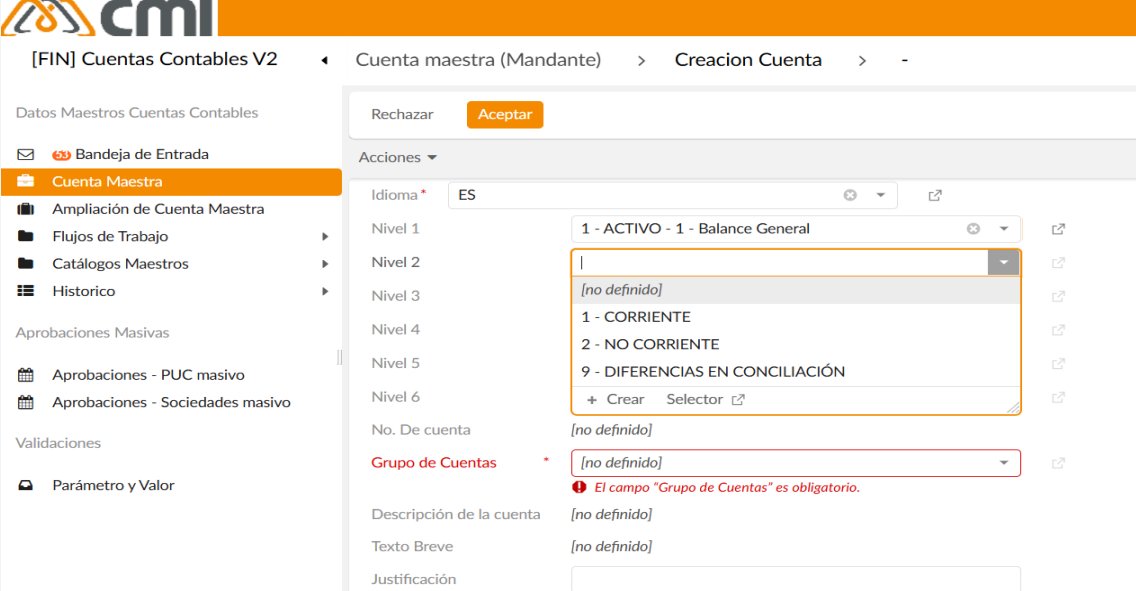
\includegraphics[width=0.8\textwidth]{NivelPUC/Creacion/ImgCreacion/CS13.png}

    \end{minipage}

\item
    \begin{minipage}[t]{\linewidth}
        Dentro el catálogo de "Nivel 3" se elige la opción correspondiente.

        \raggedright
        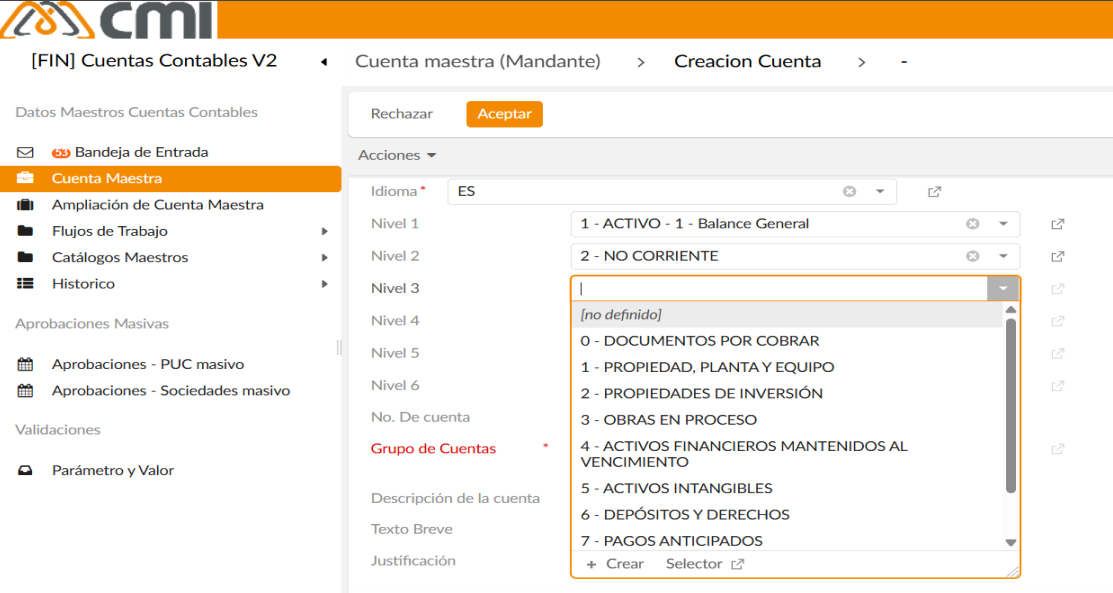
\includegraphics[width=0.8\textwidth]{NivelPUC/Creacion/ImgCreacion/CS14.png}

    \end{minipage}

\item
    \begin{minipage}[t]{\linewidth}
        Dentro el catálogo de "Nivel 4" se elige la opción correspondiente.
        
        \raggedright
        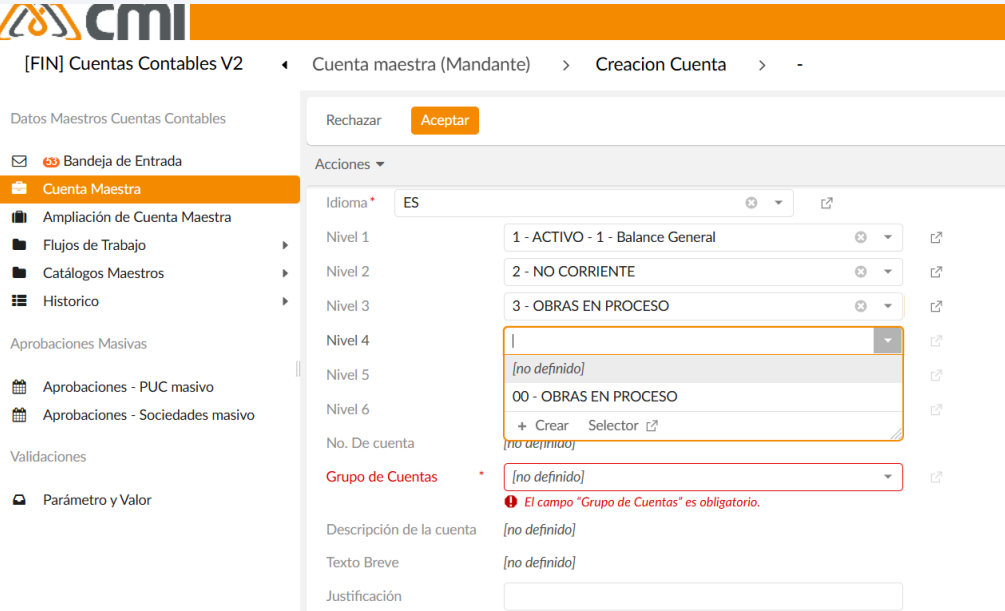
\includegraphics[width=0.8\textwidth]{NivelPUC/Creacion/ImgCreacion/CS15.png}

    \end{minipage}

\item
    \begin{minipage}[t]{\linewidth}
        Dentro el catálogo de "Nivel 5" se elige la opción correspondiente.

        \raggedright
        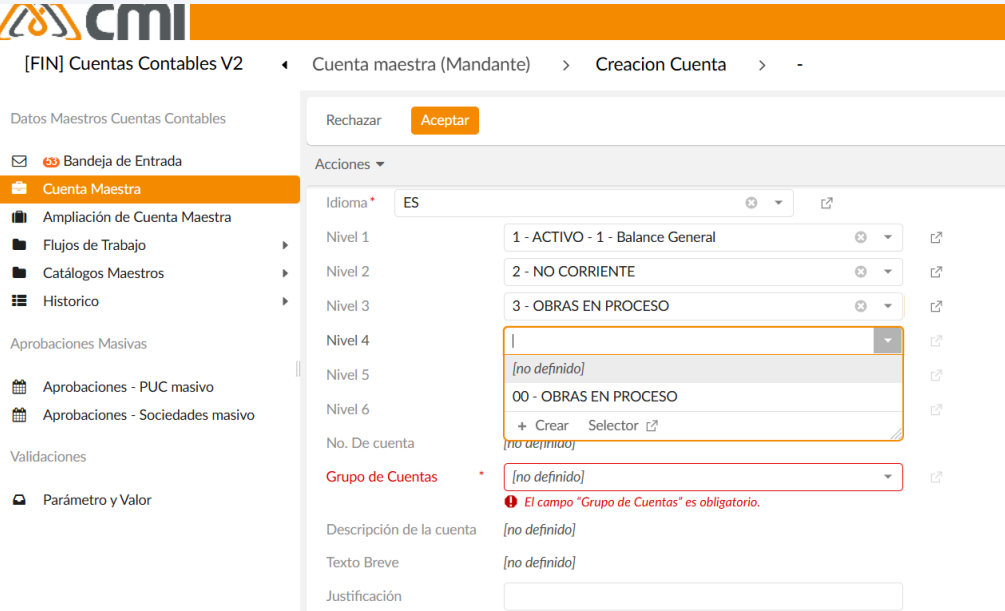
\includegraphics[width=0.8\textwidth]{NivelPUC/Creacion/ImgCreacion/CS15.png}

    \end{minipage}

\item
    \begin{minipage}[t]{\linewidth}
        Dentro el catálogo de "Nivel 6" se elige la opción correspondiente.

        \raggedright
        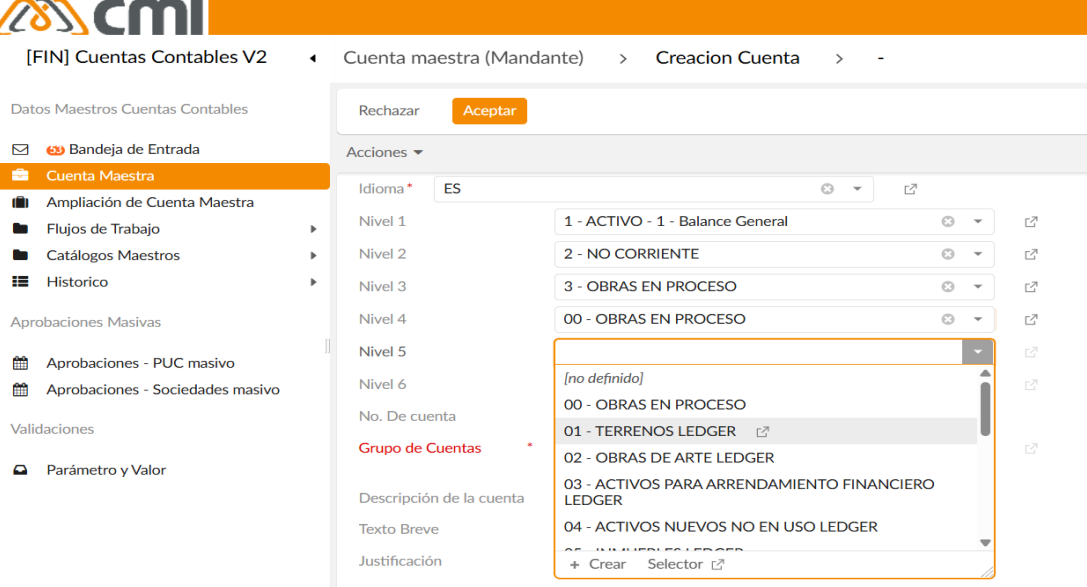
\includegraphics[width=0.8\textwidth]{NivelPUC/Creacion/ImgCreacion/CS16.png}

    \end{minipage}

\end{enumerate}




%% ### CONTRAPORTADA


% \AddToShipoutPictureBG*{%
%     \AtPageLowerLeft{%
%         
\includegraphics[width=\paperwidth,height=\paperheight]{ImagenesFormato/image3.jpg}
%     }%
% }

% \mbox{}
\newpage

\NoBgThispage
\begin{tikzpicture}[remember picture,overlay]

\node at (current page.center) {%
    
\includegraphics[
        width=\paperwidth,
        height=\paperheight
    ]{ImagenesFormato/image3.jpg}
};
\end{tikzpicture}

\end{document}